%\addtocounter{chapter}{3}%only temporary
\chapter{GA-based DSA With Basic Genetic Operators}\label{sec:Pf}
Bla Bla

\begin{figure}[!htb]
\begin{center}
%\hspace{35mm}
\vspace{-5mm}
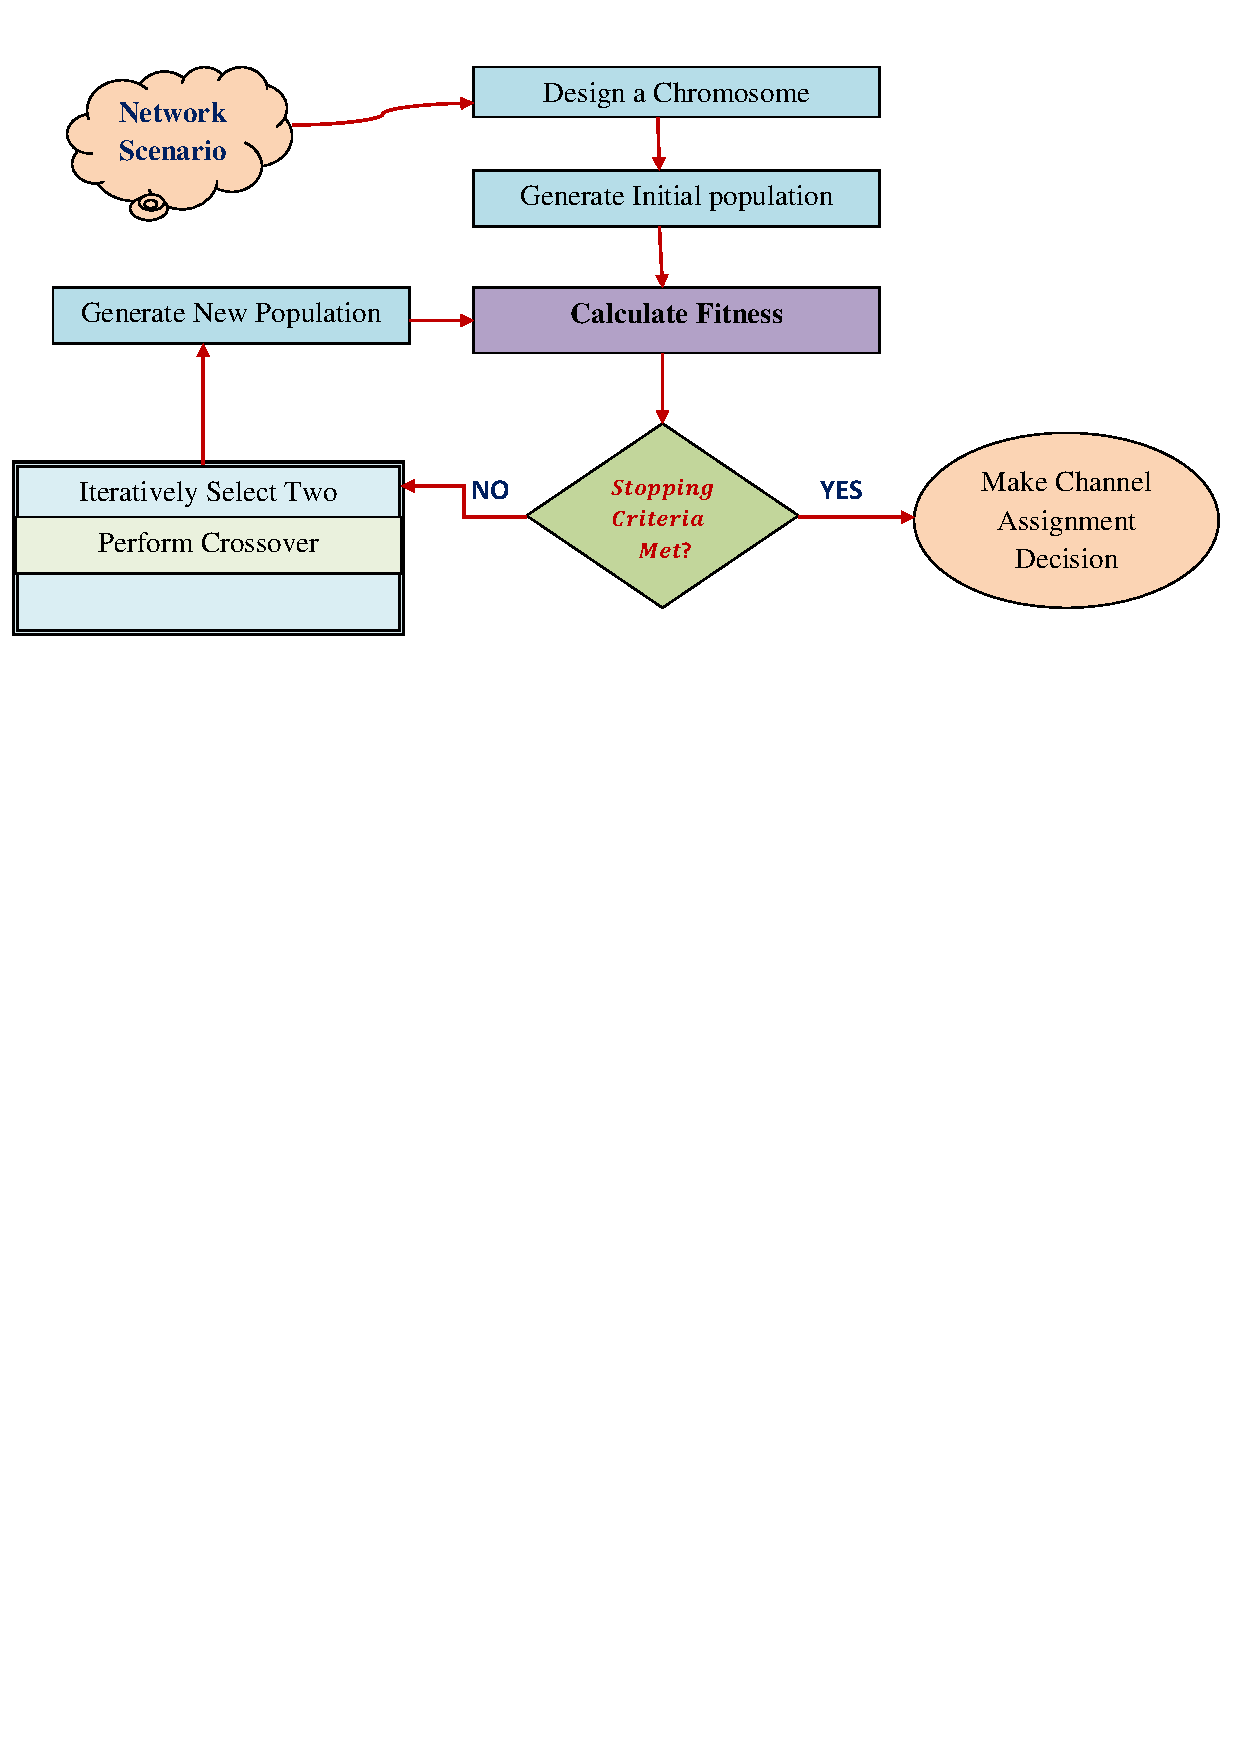
\includegraphics [scale=0.75]{algos/GA.pdf}
\vspace{-140mm}
\caption{Basic GA-based DSA}
\vspace{-3mm}
\label{GAlgo}
\end{center}
\end{figure}



\begin{table}[t]
\begin{center} \vspace{1mm}
\caption{All possible ranges of values of F(I) for $n=6$ and $n_p=2$}\vspace{-2mm}
\begin{tabular}{|c|c|c|c|}
\hline
$INP(I)$ & $IN(I)$ & \textbf{ Range of $F(I)$ }& Range of $F_1(I)$\\ \hline
\multirow{4}{*}{0} & 0 & \textbf{[1, 2]} & [1, 2]  \\ \cline{2-4}
&1 & \textbf{[1.58, 3.17]} & [2, 4] \\ \cline{2-4}
&2 & \textbf{[2, 4] }& [3, 6] \\ \cline{2-4}
&3 & \textbf{[2.32, 4.64]} & [4, 8] \\
\hline
\multirow{4}{*}{1} & 1 & \textbf{[3.17, 6.34]} & [4, 8] \\ \cline{2-4}
&2 & \textbf{[4, 8]} & [6, 12] \\ \cline{2-4}
&3 & \textbf{[4.64, 9.2]} & [8, 16] \\ \cline{2-4}
&4 & \textbf{[5.17, 10.3]} & [10, 20] \\
\hline
\multirow{4}{*}{2} & 2 & \textbf{[6, 12] }& [9, 18] \\ \cline{2-4}
&3 & \textbf{[6.97, 13.93]} & [12, 24] \\ \cline{2-4}
&4 & \textbf{[7.75, 15.5]} & [15, 30] \\ \cline{2-4}
&5 & \textbf{[8.42, 16.84]} & [18, 36] \\
\hline
\end{tabular}
%\vspace{-4mm}
\label{fitness}
\end{center}
\end{table}

\begin{figure*}[!thb]
\centering\vspace{-7mm}
\begin{tabular}{cc}
\hspace{-5mm}
        \subfigure[Ranges of $F(I)$]{%
           \label{fig:second}
           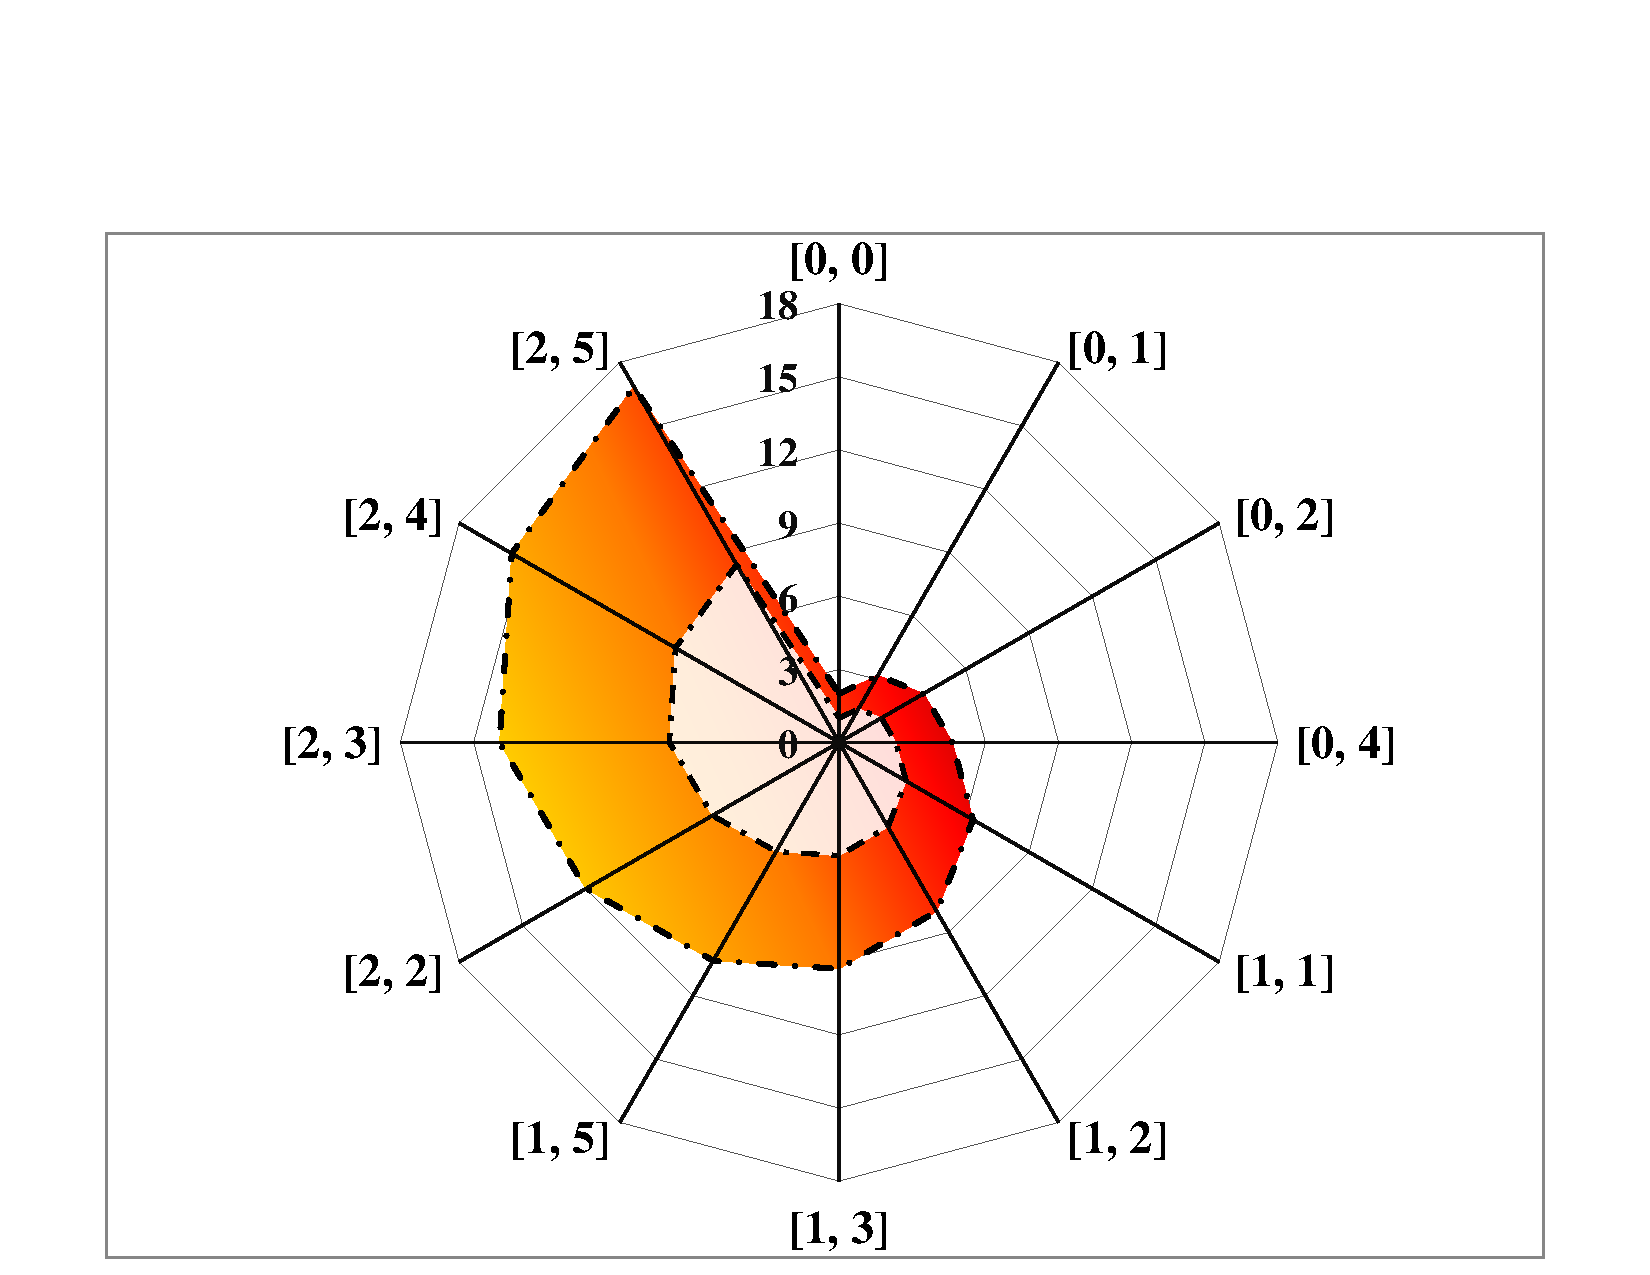
\includegraphics [width=.5\textwidth]{results/radial.pdf}
        } &
        % \vspace{-3mm}  \\
	\hspace{-10mm}
        \subfigure[Ranges of $F_1(I)$]{%
           \label{fig:second}
           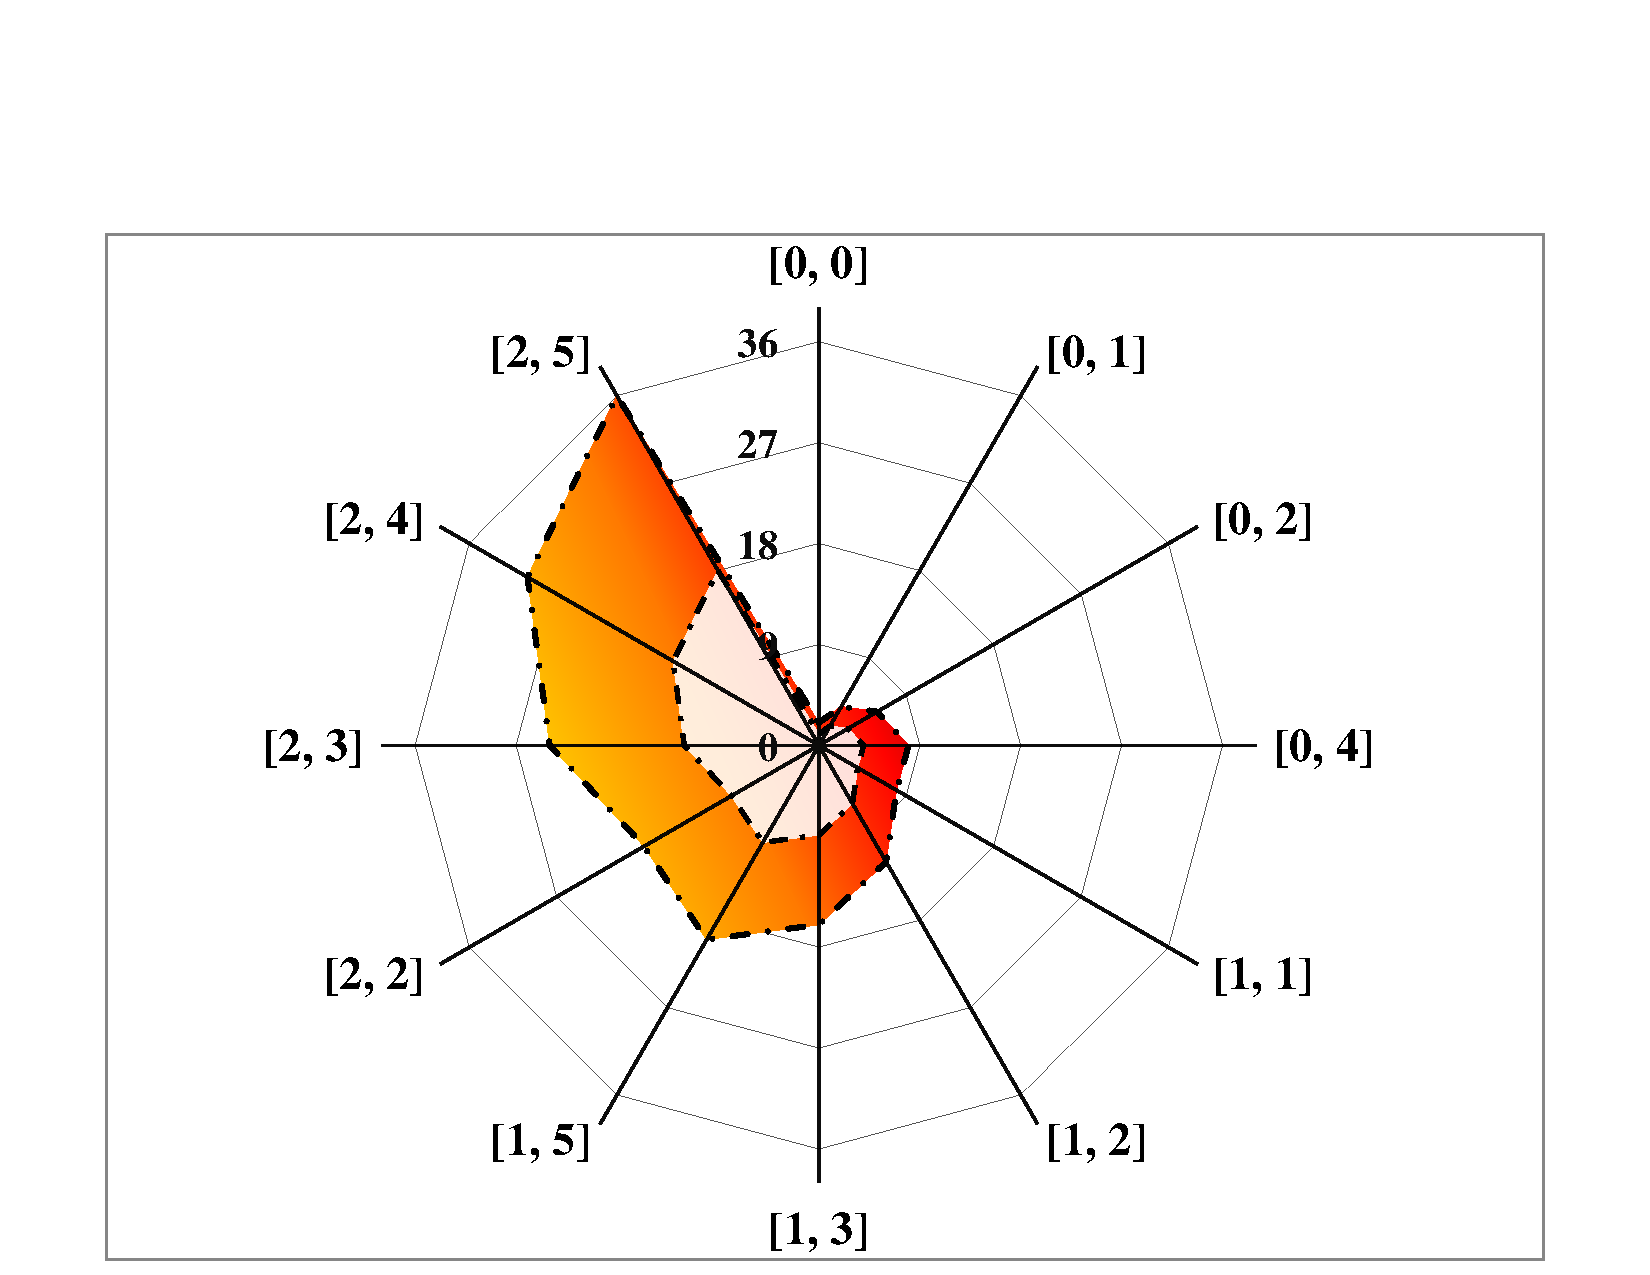
\includegraphics [width=.5\textwidth]{results/radial2.pdf}
        }
\end{tabular}
\vspace{-1mm}
    \caption{Value ranges of different fitness functions for varying combination of [INP(I), IN(I)] pairs considering $(n=6, n_p=2)$}
  %  \vspace{-5mm}
   \label{fig:radial}
%   \end{center}
 \end{figure*}



\begin{figure}[!htb]
%\begin{center}
\hspace{35mm}
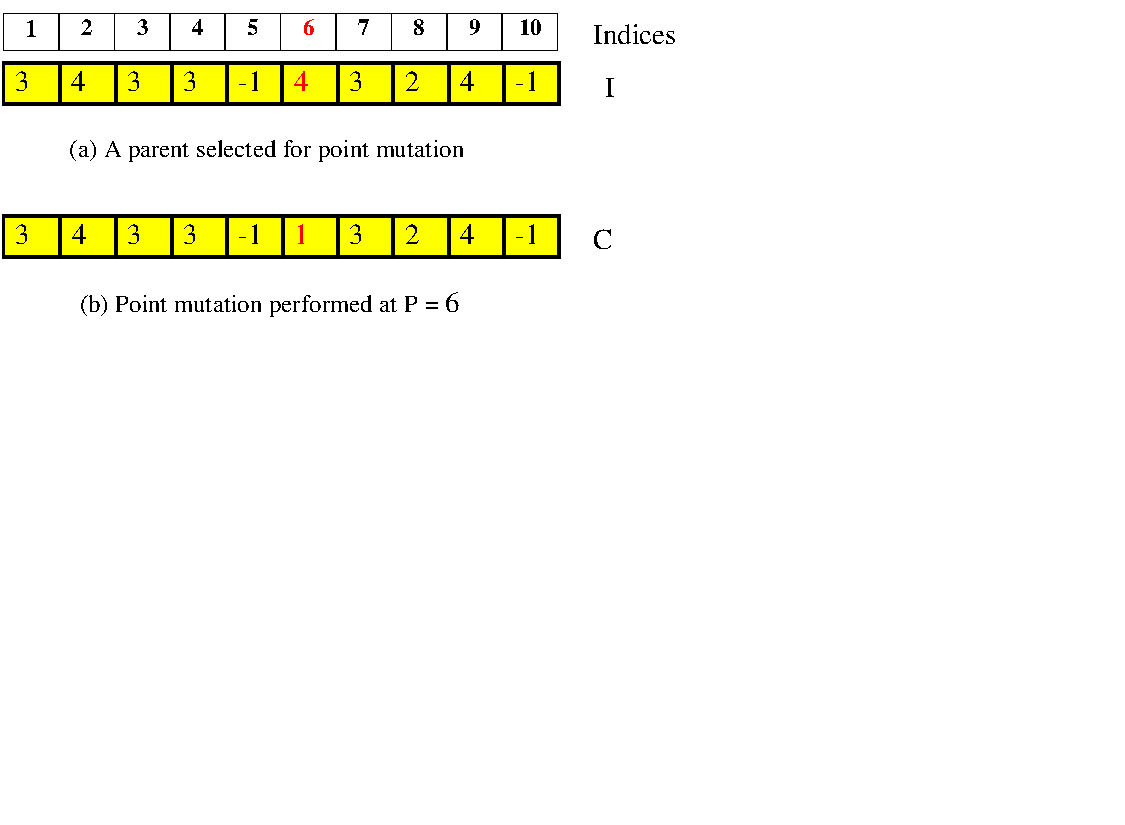
\includegraphics [scale=0.85]{figures/mute.pdf}
\vspace{-75mm}
\caption{Point mutation operation}
%\vspace{-8mm}
\label{mute}
%\end{center}
\end{figure}

\begin{center}
\begin{figure*}[!thb]
\vspace{-33mm}
\centering
\begin{tabular}{ll}

		\hspace{-15mm}
        \subfigure[T, 1-P]{
            \label{fig:first}
            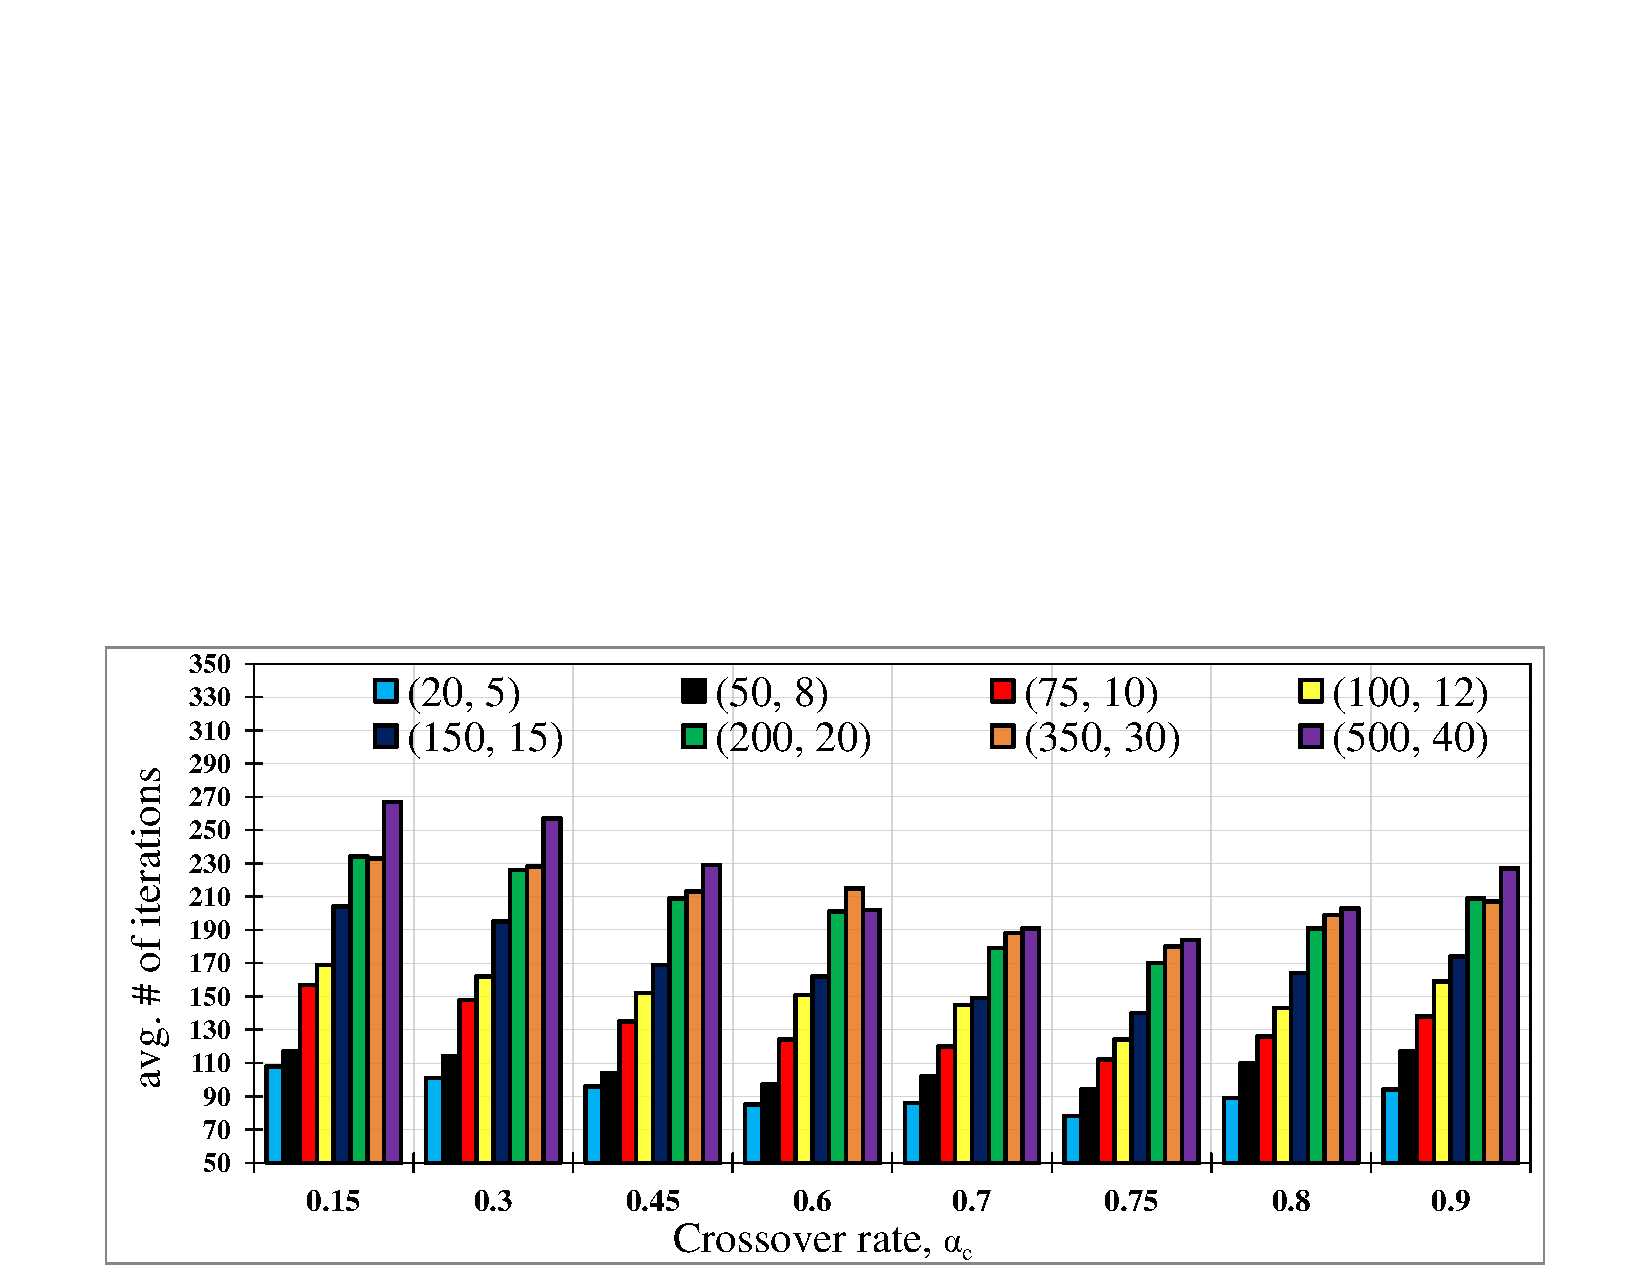
\includegraphics [width=.55\textwidth]{results/1pt.pdf} 
        }
        
        \hspace{-10mm}
        \subfigure[W, 1-P ]{%
           \label{fig:second}
           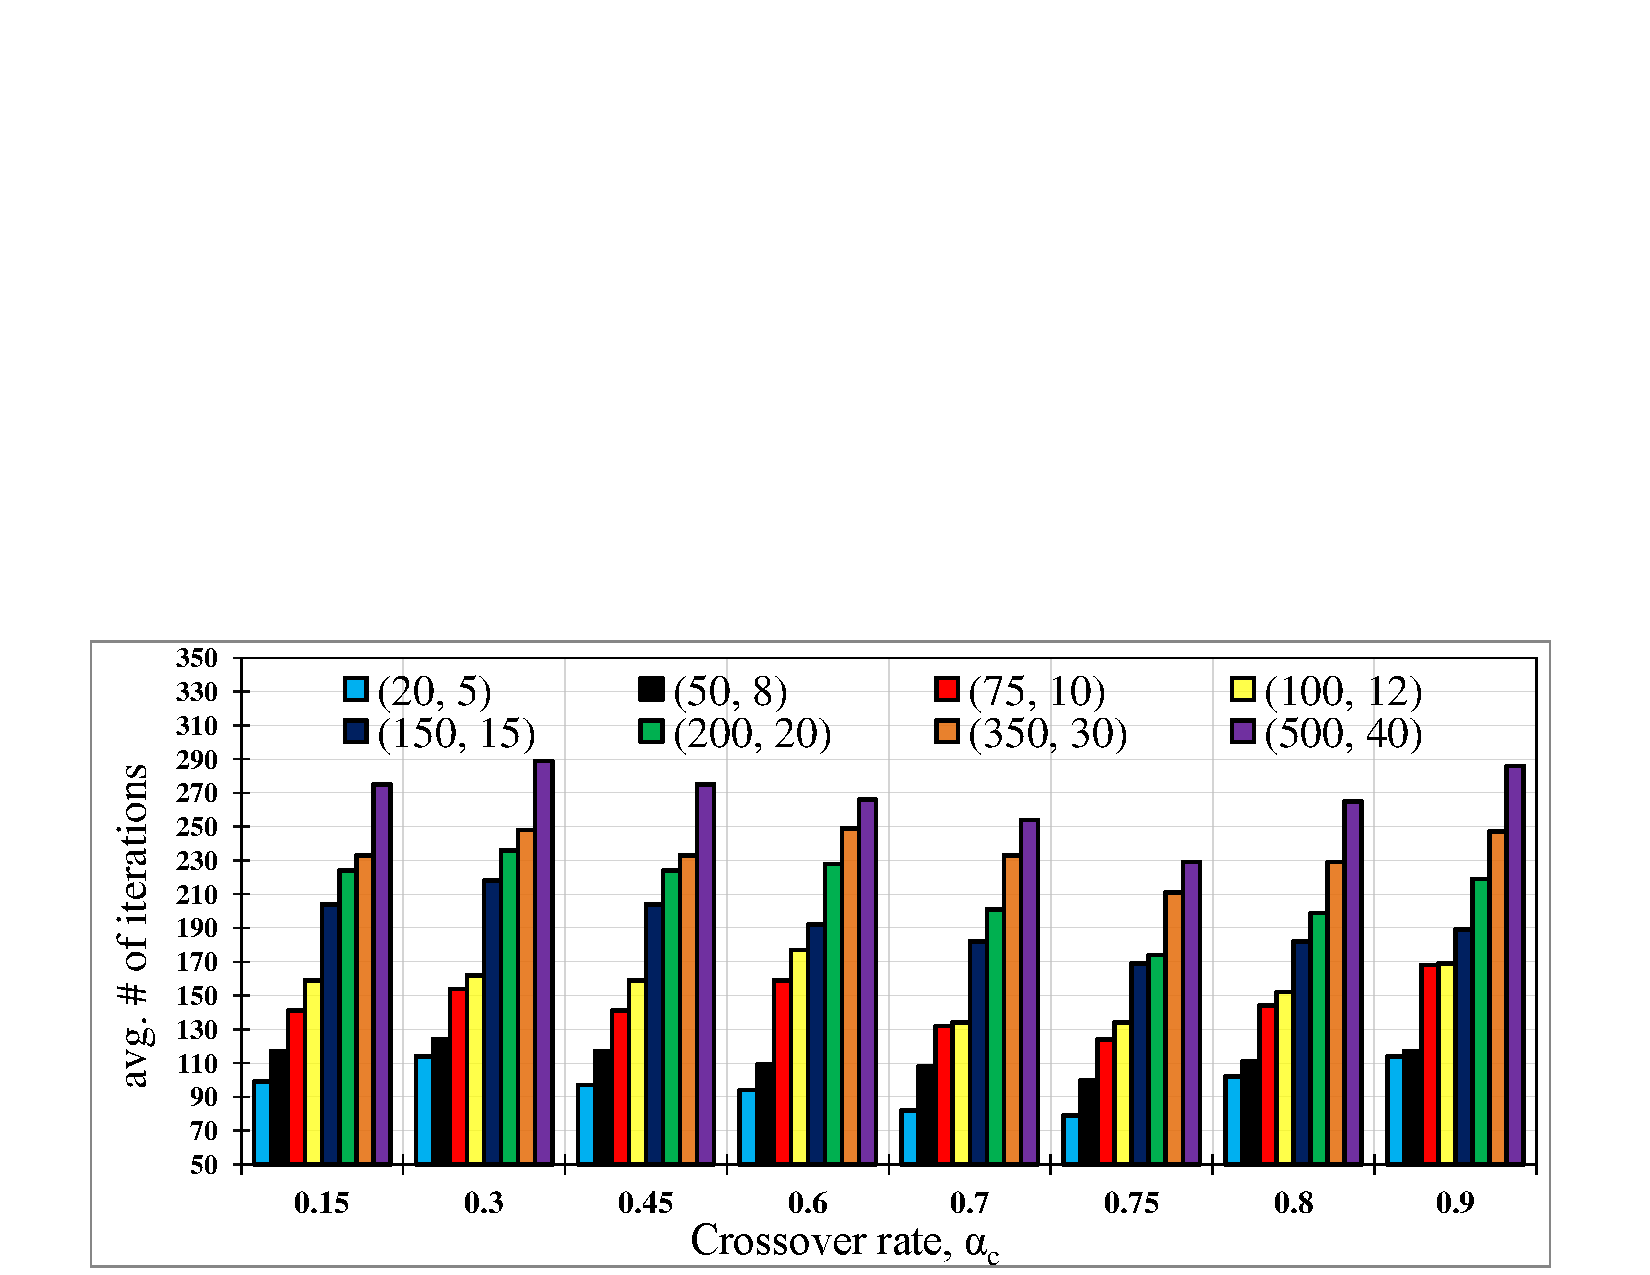
\includegraphics [width=.55\textwidth]{results/1pw.pdf}
        }
      \vspace{-30mm}	
\end{tabular}

\begin{tabular}{ll}

		\hspace{-15mm}
        \subfigure[T, 2-P]{%
          \label{fig:first}
            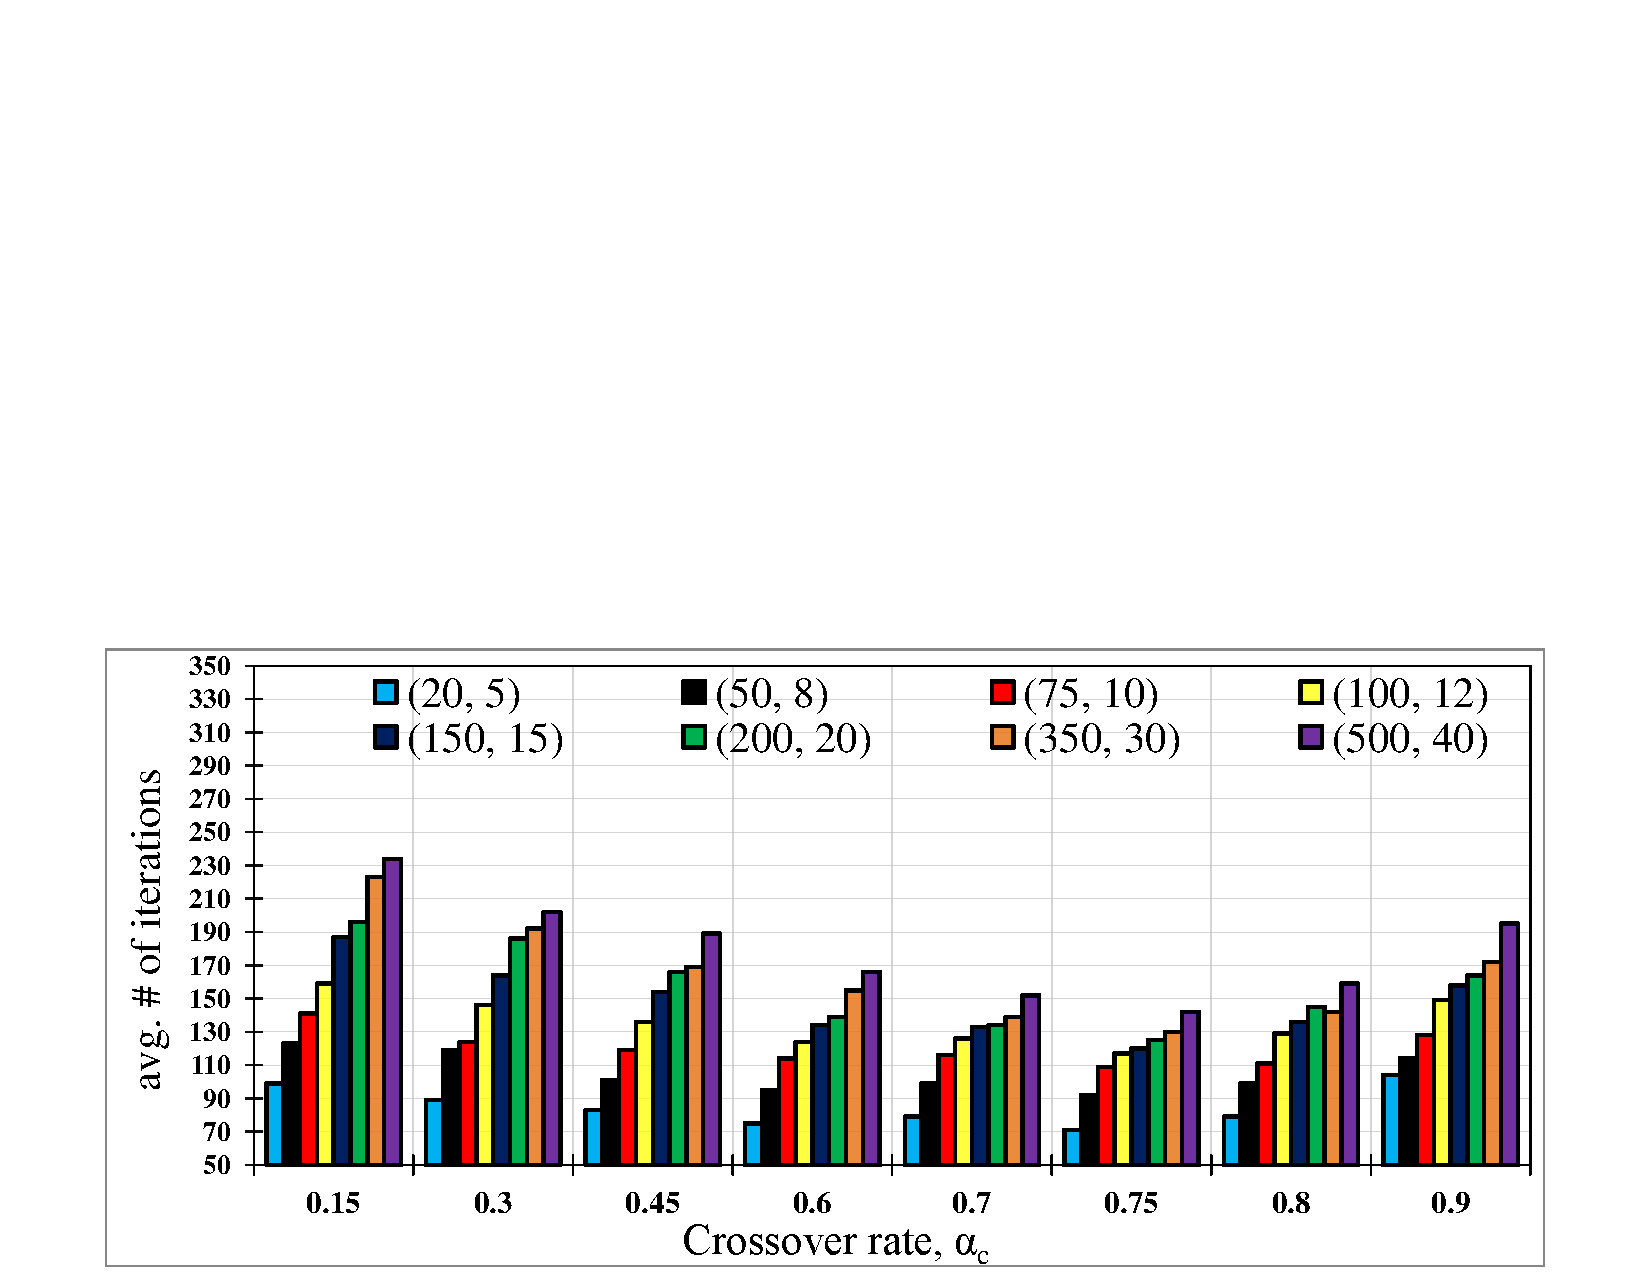
\includegraphics [width=.55\textwidth]{results/2pt.pdf} 
      }
      \hspace{-10mm}
       \subfigure[W, 2-P]{%
          \label{fig:second}
           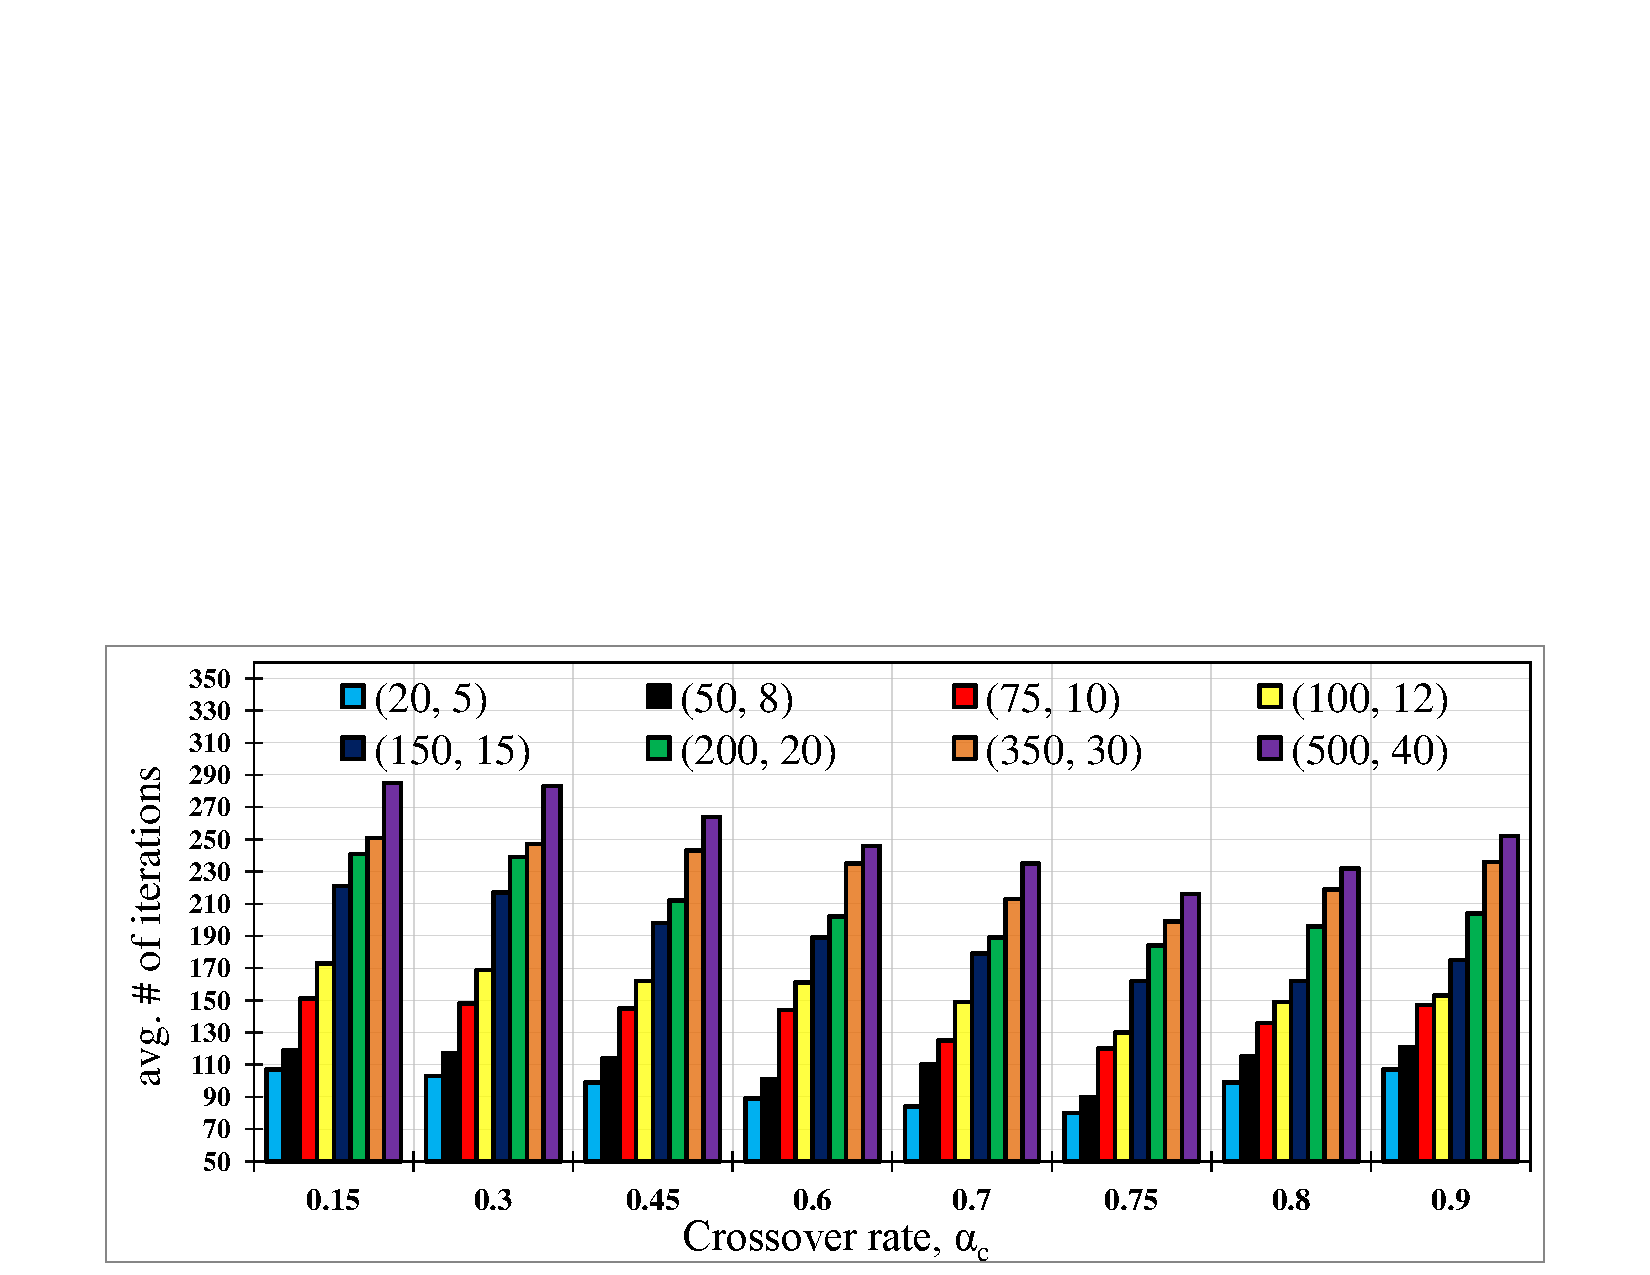
\includegraphics [width=.55\textwidth]{results/2pw.pdf} 
        }
      \vspace{-30mm}	
\end{tabular}

\begin{tabular}{ll}	
        
        \hspace{-15mm}
       \subfigure[T, U]{%
           \label{fig:first}
            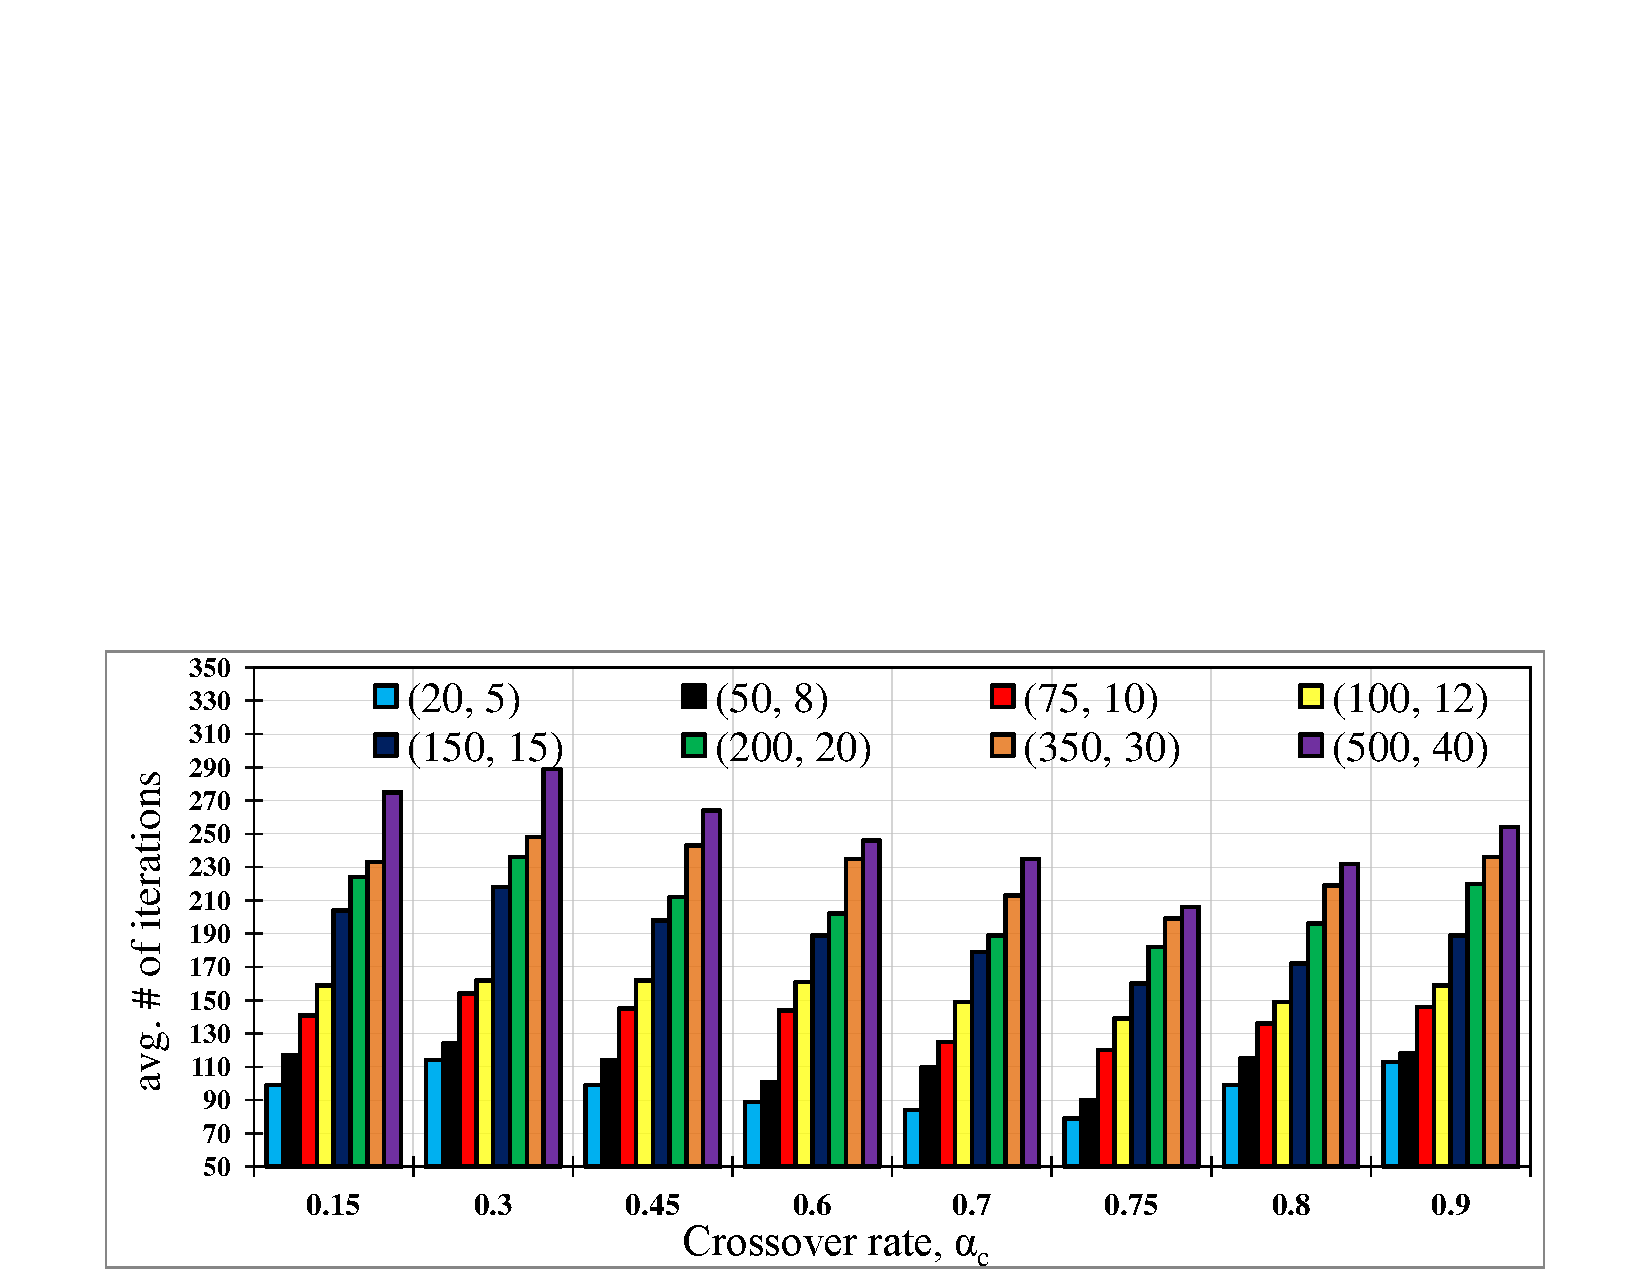
\includegraphics [width=.55\textwidth]{results/upt.pdf} 
       }
        
        \hspace{-10mm}
      \subfigure[W, U]{%
           \label{fig:second}
           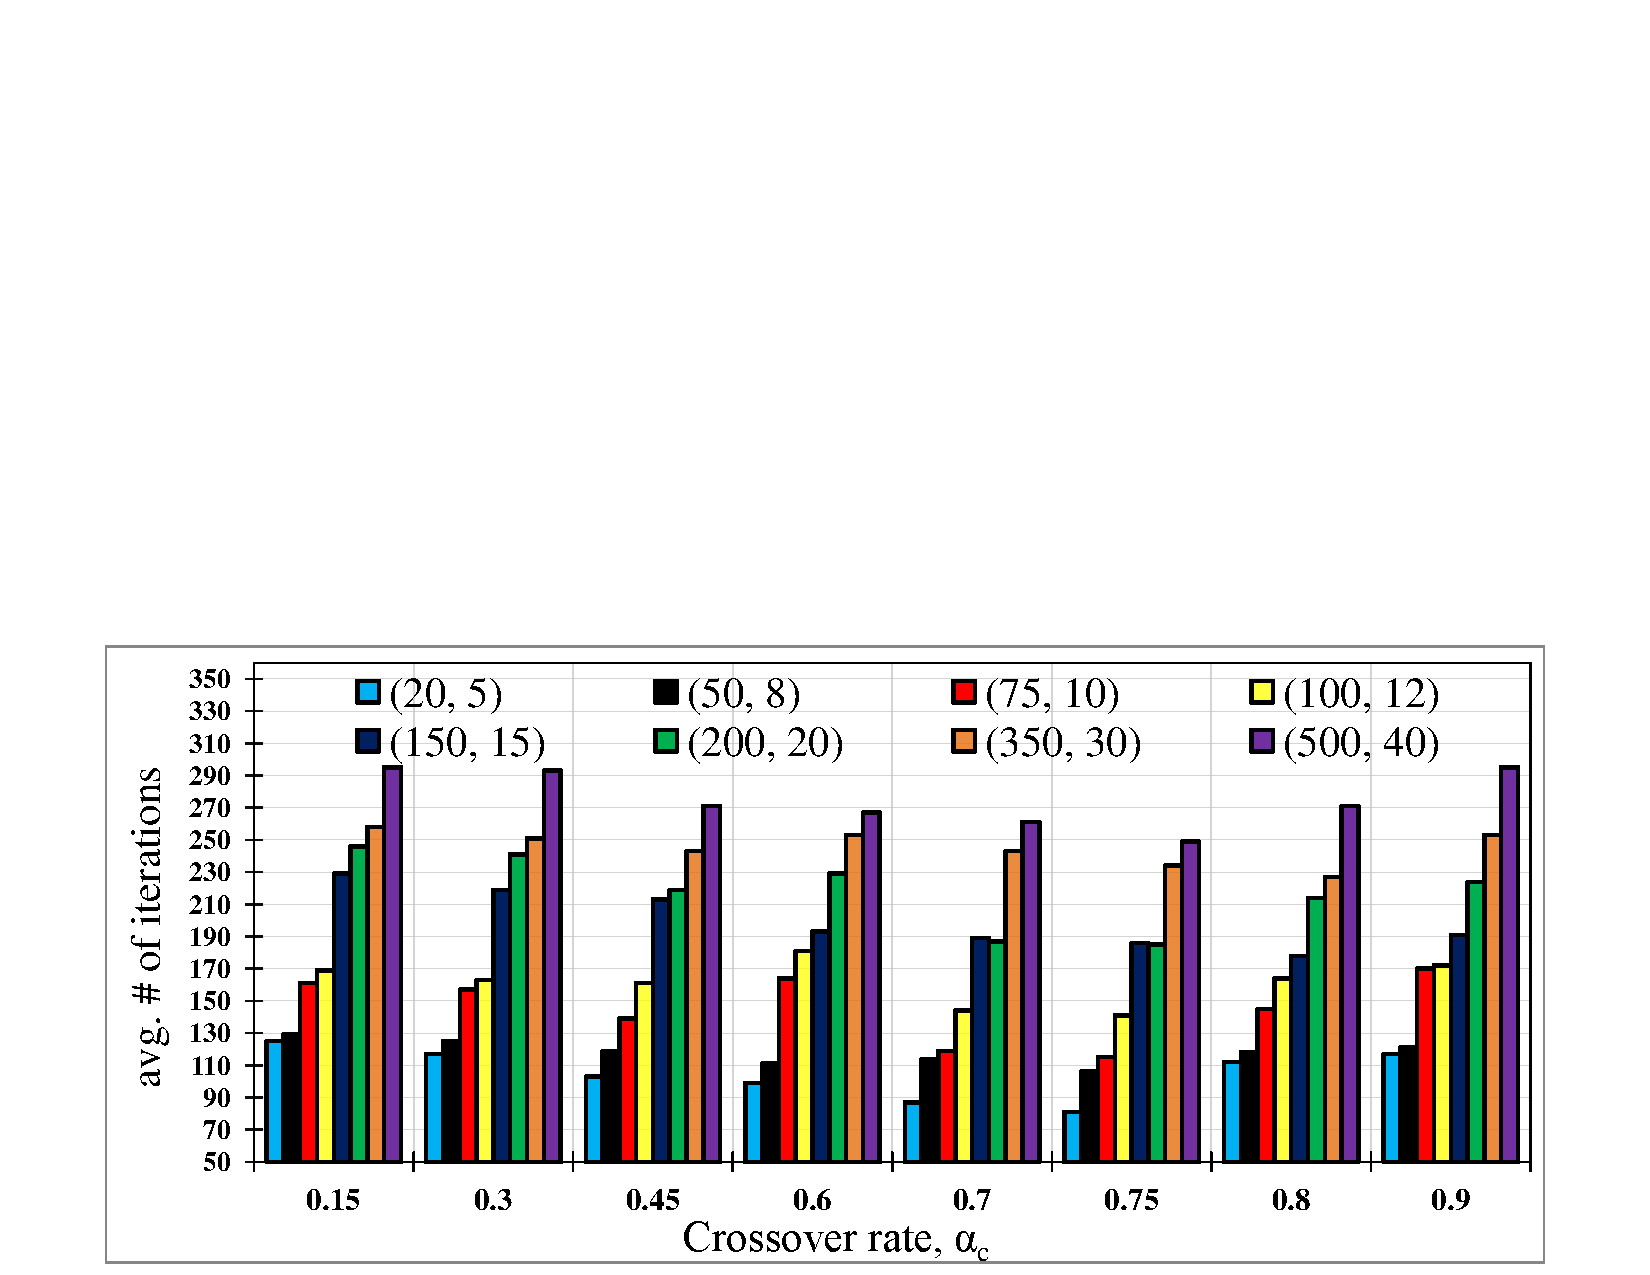
\includegraphics [width=.55\textwidth]{results/upw.pdf}
       }
		
		%\vspace{1mm}
\end{tabular}
\vspace{-1mm}
\caption{Performance of GA as DSA algorithm for different $(n, m)$ pairs with different combination of genetic operators and parameter values. Here, 1-P denotes 1-point crossover, 2-P denotes 2-point crossover, $U$ denotes uniform crossover, $T$ denotes Tournament selection, and $W$ denotes Rank-based roulette wheel selection. } %\vspace{-13mm}
   \label{fig:test3}
\end{figure*}
\end{center}  

%\vspace{-5mm}

\begin{center}
\begin{figure}[h]
\vspace{-26mm}
\centering
\begin{tabular}{ccc}

		\hspace{-15mm}
		 \subfigure[Avg. number of iterations needed for convergence]{
           \label{fig:second}
           
           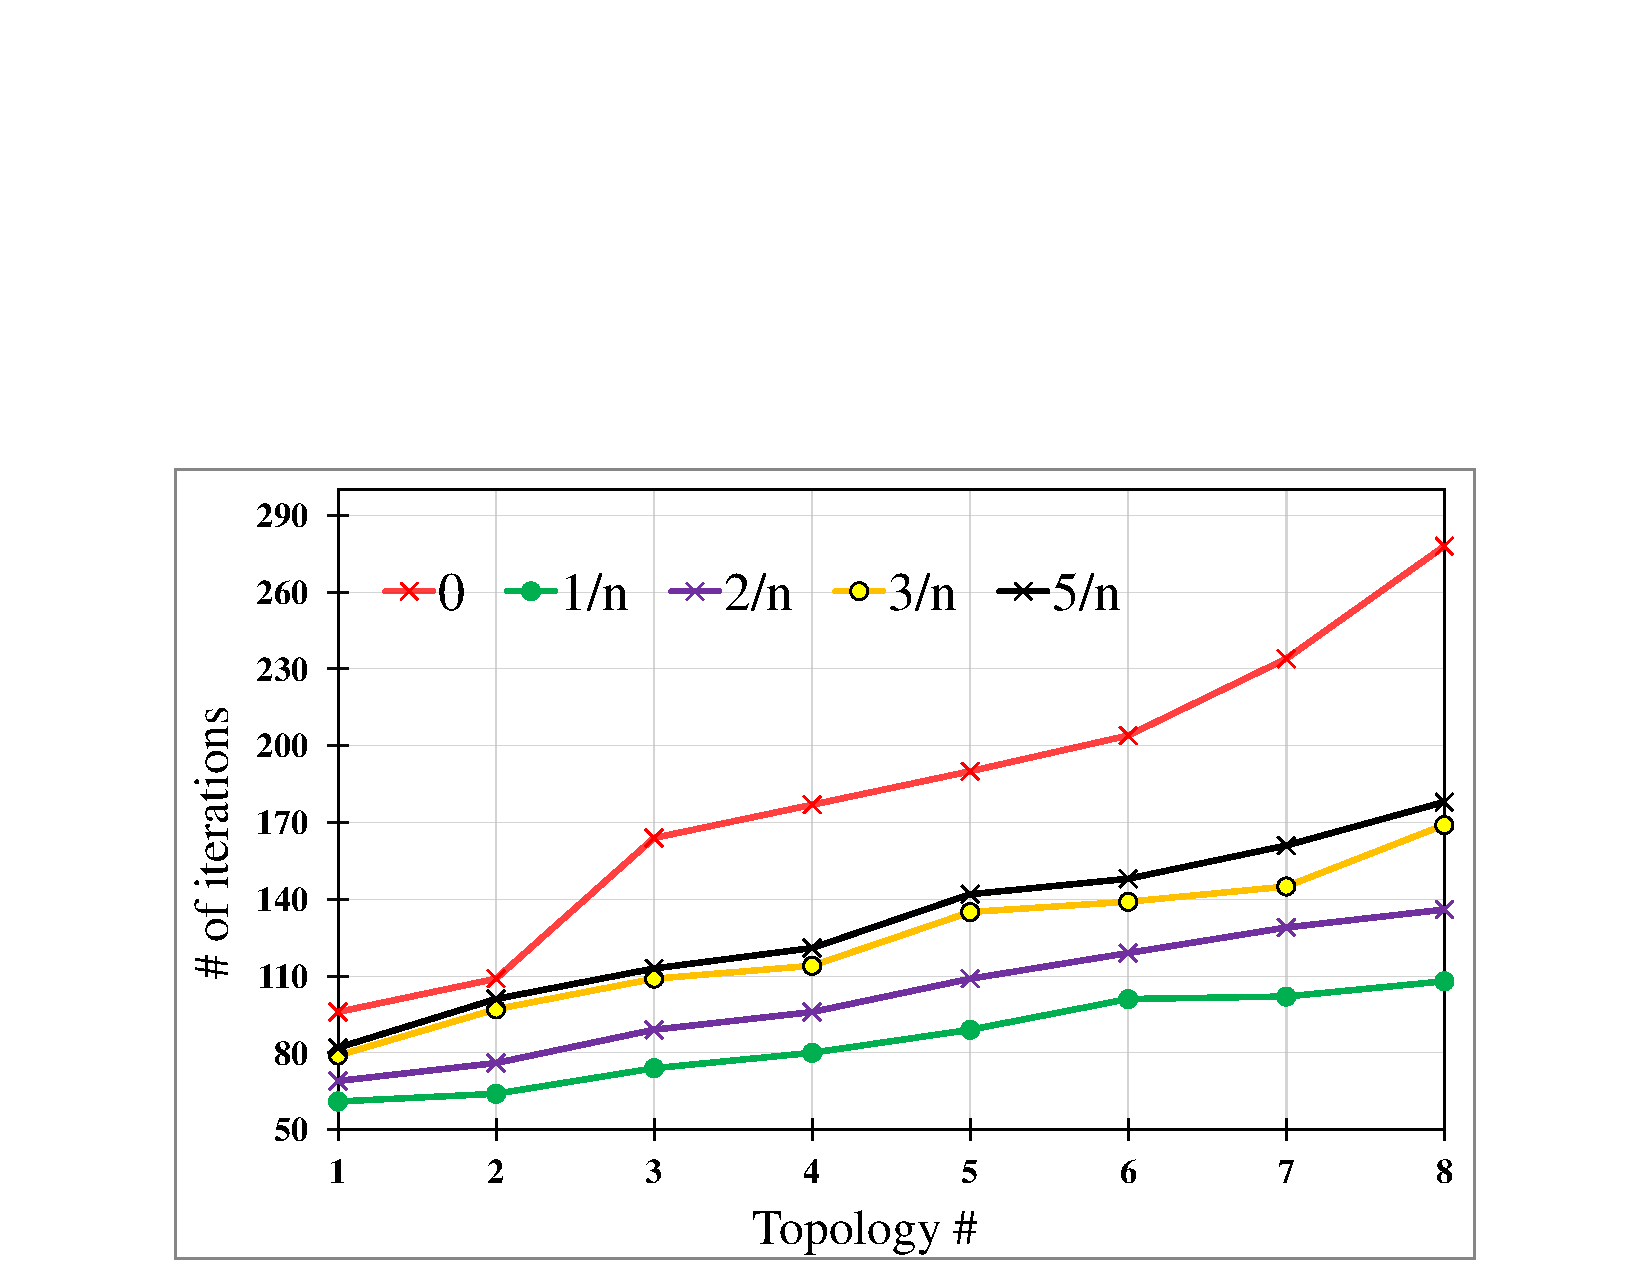
\includegraphics [width=.6\textwidth]{results/muavg.pdf}
         %  \vspace{-40mm}
        }
   %     \vspace{-20mm}
   %         \\
            
       \hspace{-15mm}
       
          \subfigure[Probability of successful convergence]{
            \label{fig:first}
            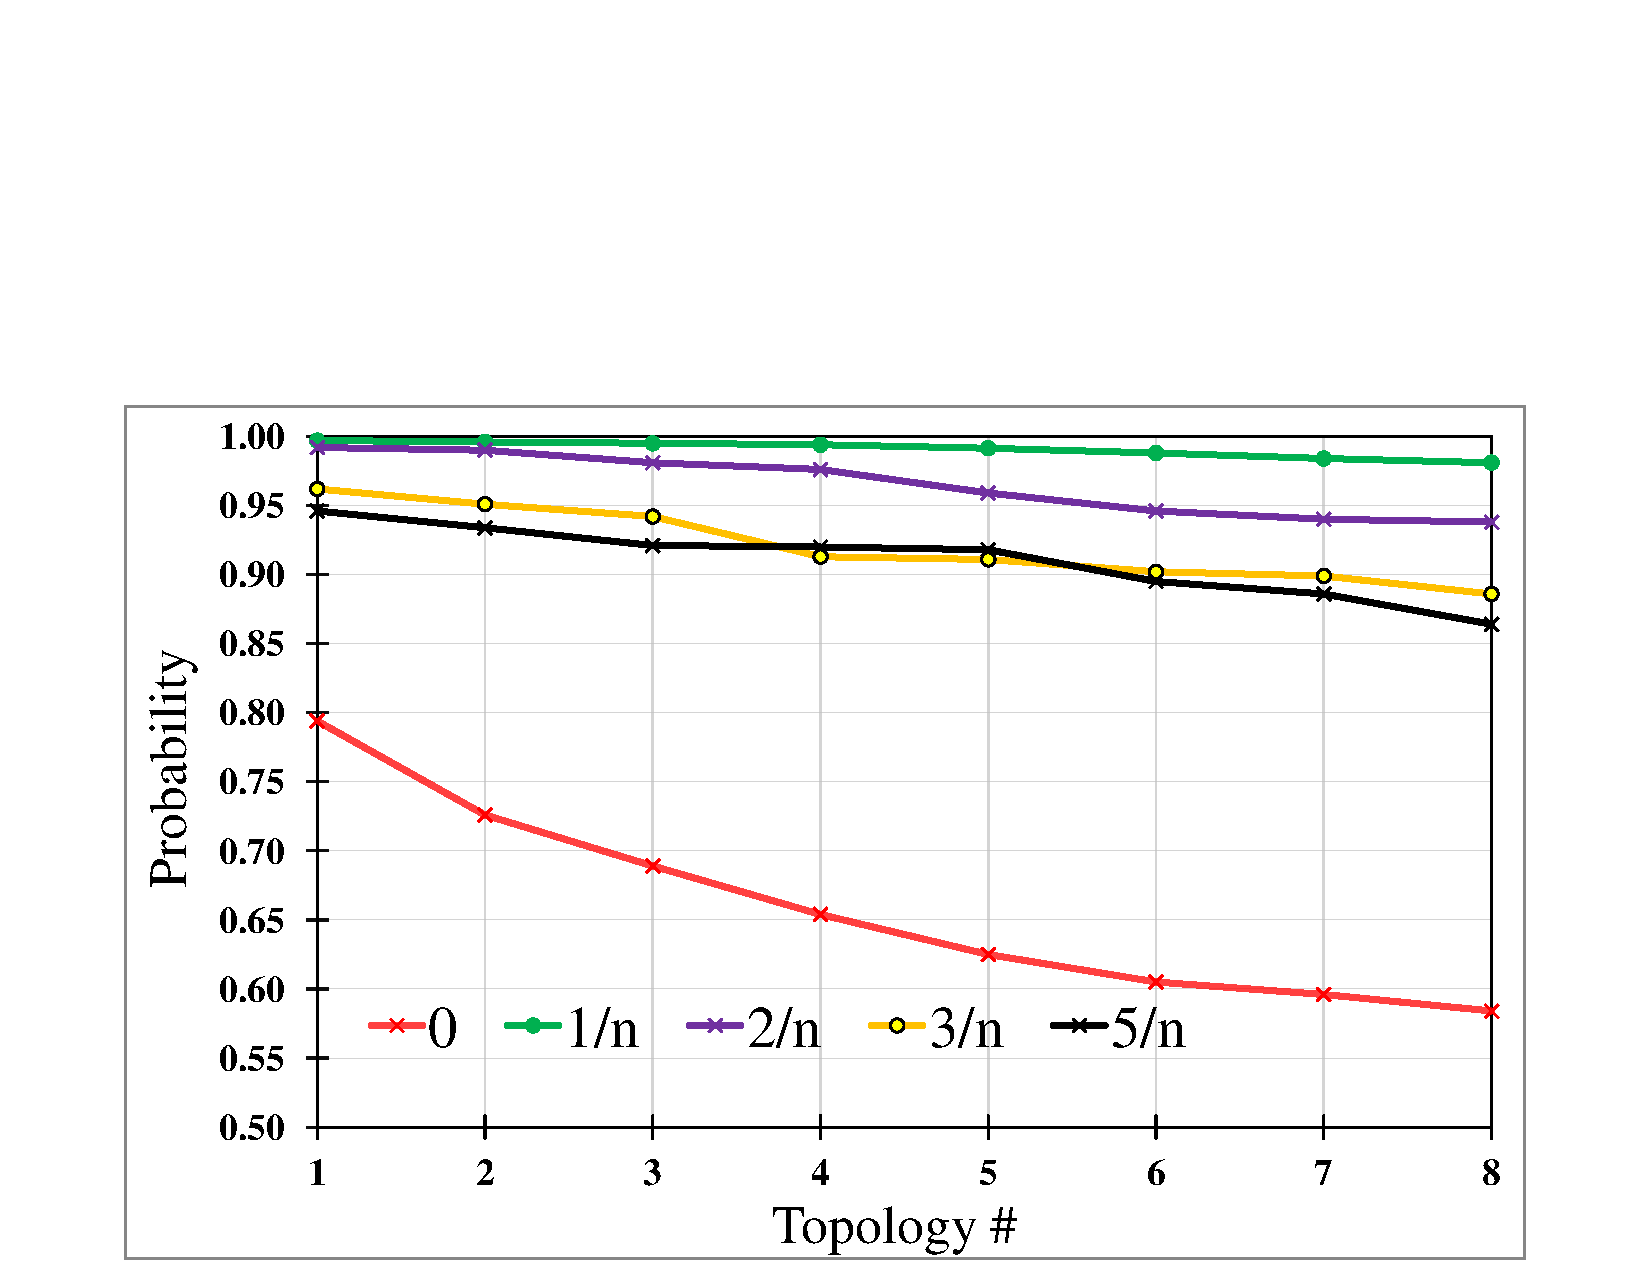
\includegraphics [width=.56\textwidth]{results/murate.pdf} 
        } \vspace{-18mm}
       \\
    %    \hspace{5mm}
       
        \subfigure[Overall convergence rate ($C_{rate}$)]{
           \label{fig:second}
           
           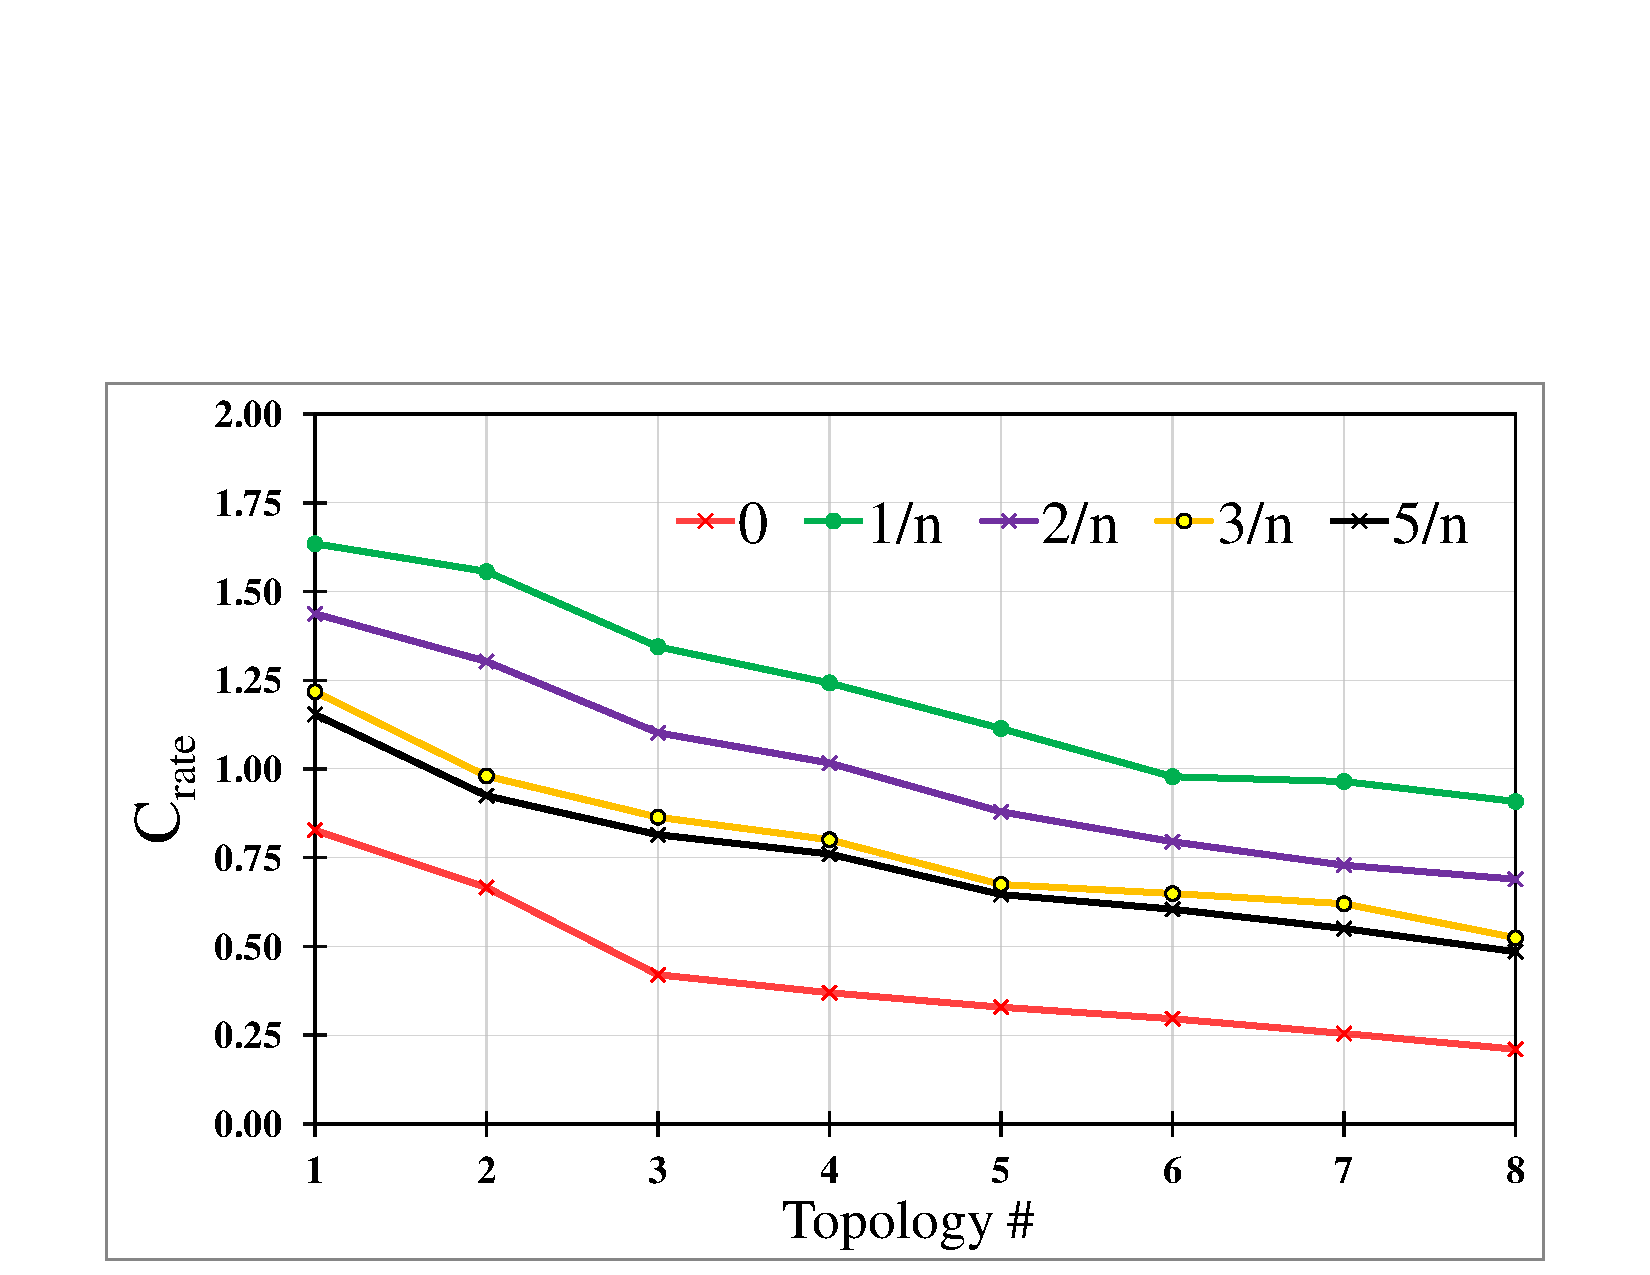
\includegraphics [width=.6\textwidth]{results/ovrate.pdf}
        }
    %  \vspace{-10mm}	
\end{tabular}
%\vspace{-1mm}
\caption{Impact of mutation rate ($\alpha_m$) on convergence over varied network topologies} %\vspace{-6mm}
   \label{fig:mut}
\end{figure}
\end{center}  

%\vspace{-12mm}
